%%---------------------------------------------------------------------------%%
\section{Results and Discussions}
\label{sec:discuss}
The pressure change through various reactor components is a crucial parameter to be considered in designing the SFR system. Due to the novelty of the proposed concept, many of its components do not have readily applicable correlations and the analysis will rely more heavily on the CFD result for accurate pressure change predictions. To demonstrate how the related design tasks can be supported by the state-of-the-art CFD flow solver, Nek5000, two case studies are to be presented in this work. The first problem investigates the jet flow exiting the axial neutron reflector channels and mixing within an upper channel. The objective here is to evaluate the pressure loss during this process given different flow conditions in terms of the Reynolds numbers. The second case study will focus on the flow entering the fuel bundle. A simplified 7-pin bundle is first studied before moving on to the realistic 217-pin bundle. The related geometry is split into two subdomains to test the NekNek coupling capability. Meanwhile, an integral domain case is also computed as a reference for the NekNek results.  


\subsection{Case study I: flow exiting the axial neutron reflector}
\label{sec:results1}

The computational domain used in the first case study is illustrated in Figure~\ref{fig:reflector}, which consists of three semi-circular inlet channels inside the reflector and a wider vertical hexagonal channel above the reflector. The inlet semi-circular channels have a 2.5 cm nominal radius while the full domain height is 18.4 cm. Both the upper and inlet channels are extruded. The extrusion of the upper domain helps avoid the recirculation issue at the outlet boundary. Meanwhile, the elongated inlet allows a fully developed turbulent inflow produced by the recycling velocity boundary condition. Three Reynolds numbers are considered, including 20,000, 50,000 and 900,000. Since the non-dimensional calculations are carried out here, the increase of Reynolds number is achieved by decreasing the flow viscosity. 

\begin{figure}[!ht]
\centering
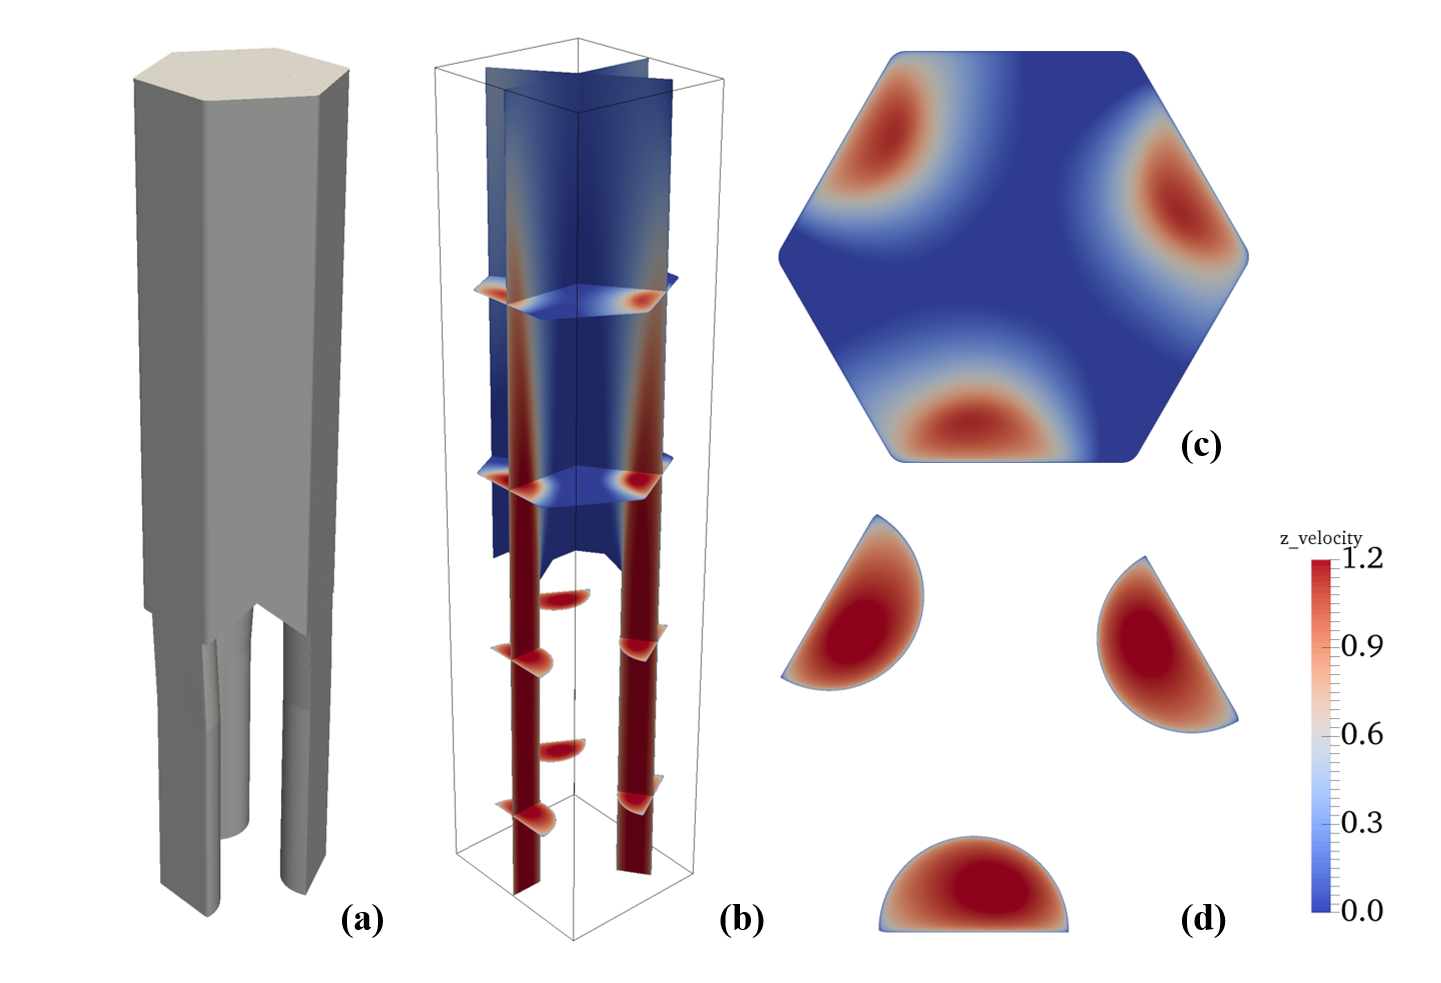
\includegraphics[width=0.8\textwidth]{./figures/reflector_domain.png}
\caption{The computational domain and steady-state velocity fields at Re of 20,000: (a) the side view; (b) the velocity fields on various cut planes; (c) a cut plane at the upper channel; (d) a cut plane over the reflector/inlet legs. }
\label{fig:reflector}
\end{figure}


The distributions of velocity, TKE ($k$) and turbulence dissipation frequency ($\omega$) are presented in Figure~\ref{fig:reflector_vel}, Figure~\ref{fig:reflector_tke}, and Figure~\ref{fig:reflector_omega} respectively. 
Overall, the turbulent flow displays similar profiles at the three Reynolds numbers. Some subtle difference is observed in the velocity profile. For instance, as shown in Figure~\ref{fig:reflector_vel}, the wake propagates longer with a higher Re. Also, the flow re-circulation is captured with negative streamwise velocity observed right after the joint region between the reflector channel and the upper channel. 
A high TKE region is noticed in the upper channel, of which the shape coincides with that the velocity profile. It indicates that a strong mixing process is going on when the jet comes out from the reflector into the upper space. As for the turbulence dissipation frequency, it is noticeably higher in the near wall region as well as where the strong mixing takes place. Again, all the calculations are done in a non-dimensional manner, and the slightly decrease in maximum TKE in Figure~\ref{fig:reflector_tke} should not be confused as the decrease in the actual TKE for higher Reynolds numbers. 
In all simulations, the $y^+$ value is monitored and ideally the closest layer of GLL points should be within $y_p^+ < 1$. So far, this restriction is only strictly kept in the case with Re of 20K. Appropriate boundary layer mesh refinement may be needed for high Re cases in the future. 

\begin{figure}[!ht]
\centering
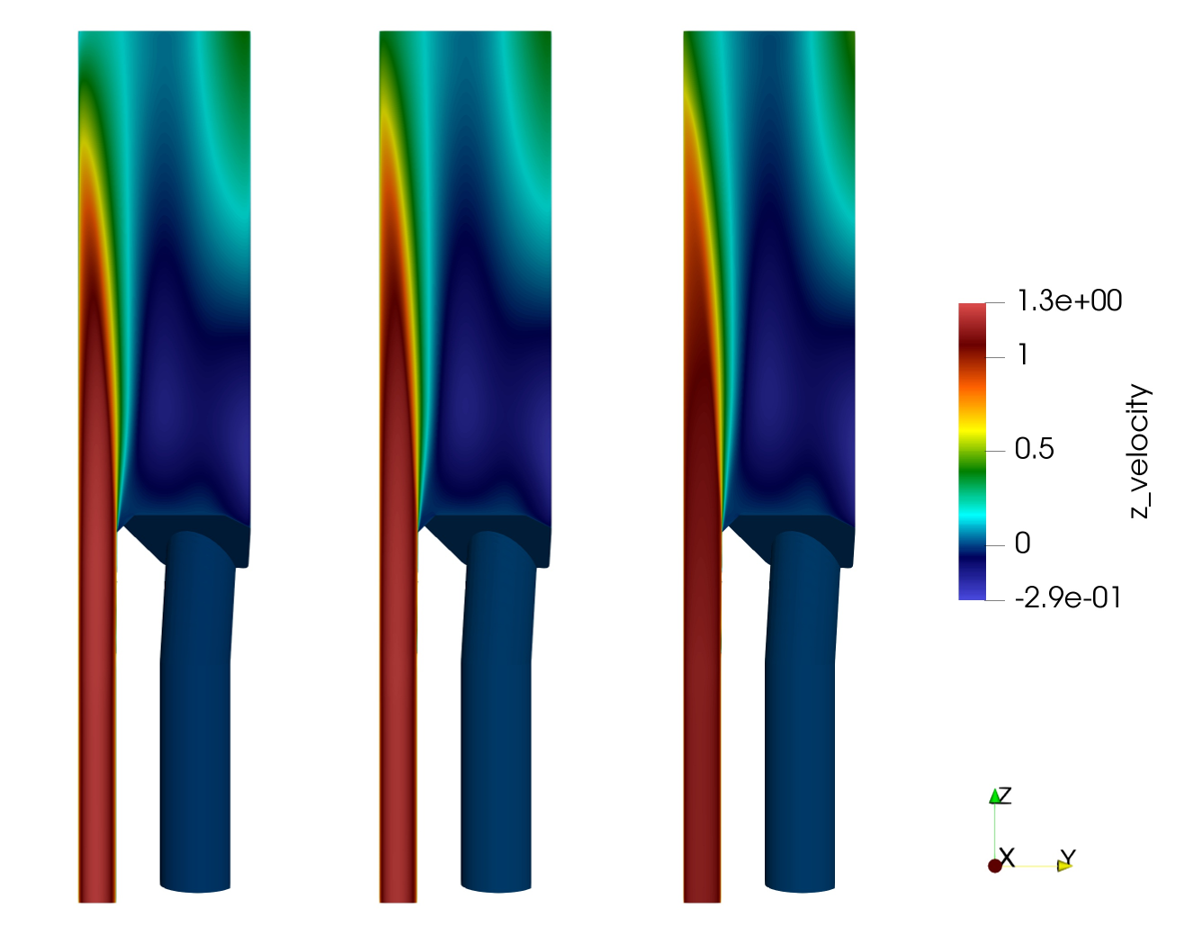
\includegraphics[width=0.8\textwidth]{./figures/reflector_vel.png}
\caption{The steady state streamwise velocity profiles at Re = 20,000, 50,000, 900,000 (from left to right). }
\label{fig:reflector_vel}
\end{figure}

\begin{figure}[!ht]
\centering
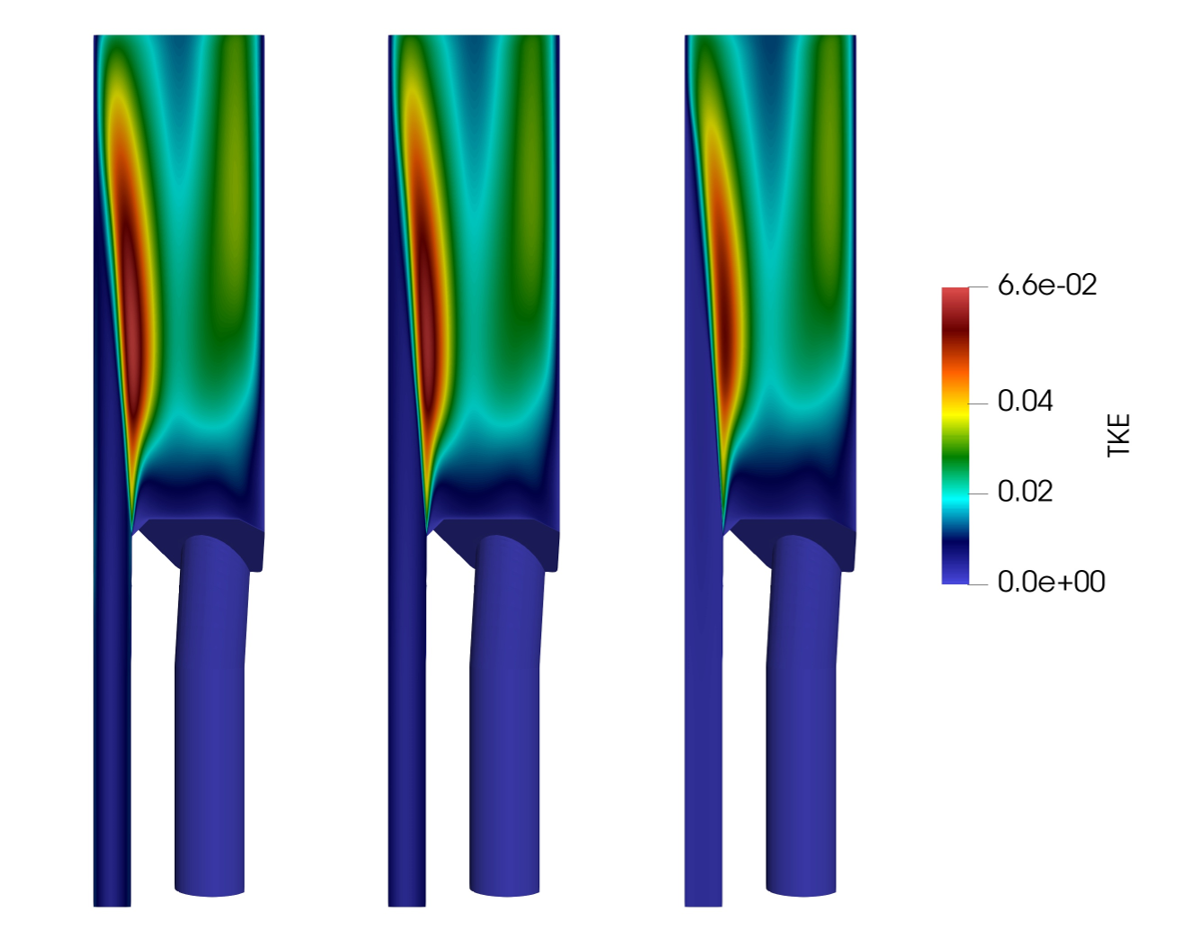
\includegraphics[width=0.8\textwidth]{./figures/reflector_tke.png}
\caption{The steady state turbulent kinetic energy profiles at Re = 20,000, 50,000, 900,000 (from left to right). }
\label{fig:reflector_tke}
\end{figure}

\begin{figure}[!ht]
\centering
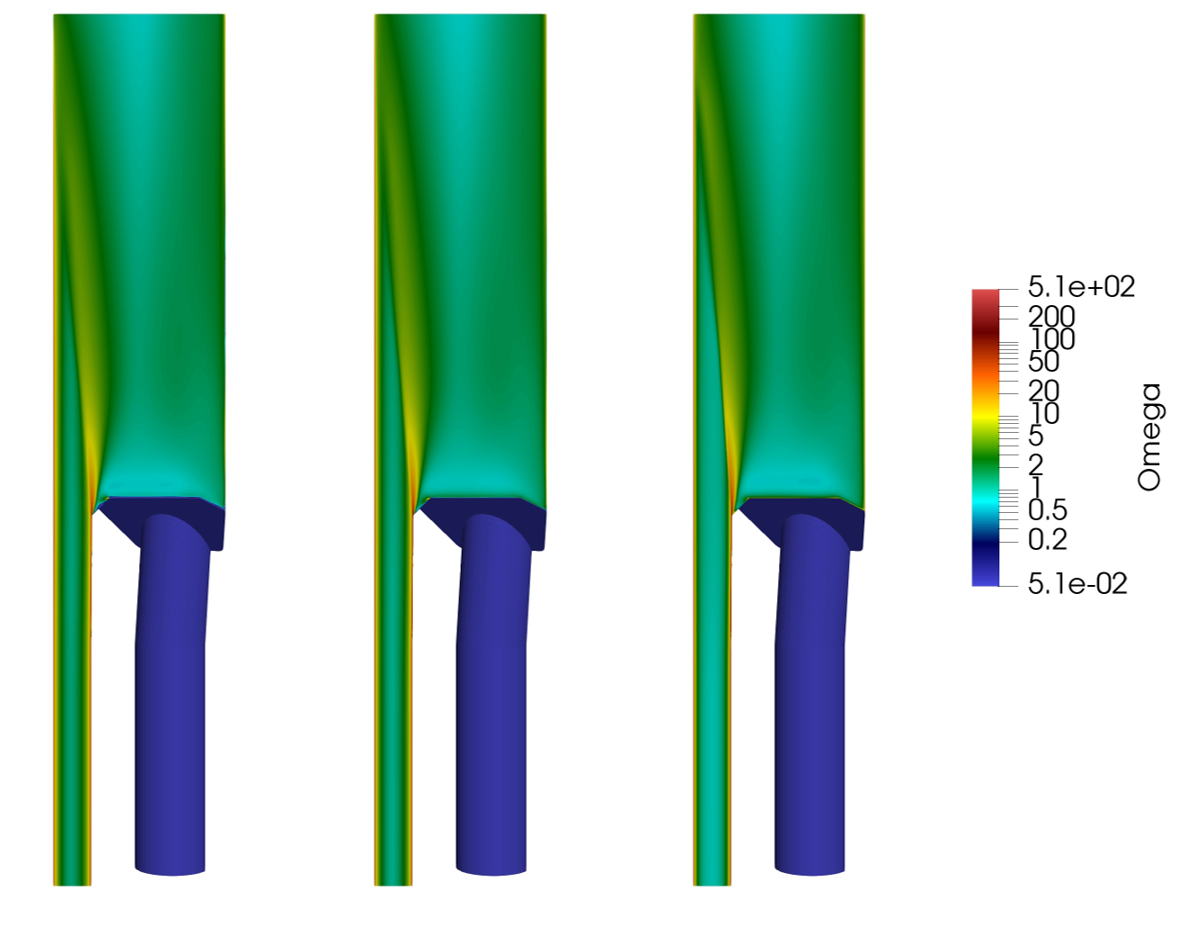
\includegraphics[width=0.8\textwidth]{./figures/reflector_omega.png}
\caption{The steady state turbulence dissipation frequency profiles at Re = 20,000, 50,000, 900,000 (from left to right) with a log scale. }
\label{fig:reflector_omega}
\end{figure}

To quantify the pressure change as the flow moves out of the semi-circular channels into a wider upper channel, the area-averaged flow quantities are first extracted at both the domain inlet and outlet. For example, the average pressure and streamwise velocity at the inlet are computed as follows: 

\begin{equation}
    P_{in} = \frac{1}{A_{in}} \oint P \cdot dA_{in}
\end{equation}

\begin{equation}
    u_{in} = \frac{1}{A_{in}} \oint u \cdot dA_{in}
\end{equation}

A pressure difference is readily obtained by subtracting the inlet pressure from the outlet pressure (i.e. $\Delta P_t = P_{out} - P_{in}$). The pressure change in the current domain has two important contributors, the wall friction effect and the Bernoulli effect due to the change of channel shape. For the incompressible flow, the Bernoulli principle can be expressed by the equation below: 

\begin{equation}
    \frac{u_{in}^2}{2} + gz_{in} + \frac{P^\prime_{in}}{\rho} = \frac{u_{out}^2}{2} + gz_{out} + \frac{P^\prime_{out}}{\rho}
\end{equation}


where $P^\prime_{in}$ and $P^\prime_{out}$ are theoretical inlet and outlet pressures if the wall friction is assumed to be zero or the Bernoulli effect is the only contributor of pressure change. It is straightforward to get Eq. (\ref{eqn:dpb}) based on the energy conservation. The mean flow slows down as it moves from the narrow passage of the semi-circular channels into a wider plenum. The gravitational acceleration ($g$) is zero in all cases, so the pressure change due to Bernoulli effect can be estimated by 

\begin{equation}
\label{eqn:dpb}
    \Delta P_B = P^\prime_{out} - P^\prime_{in} = \frac{\rho ( u_{in}^2 - u_{out}^2 )}{2} 
\end{equation}

In reality, the wall friction would always induce additional pressure loss. Then the pressure change due to the wall friction is given by 

\begin{equation}
    \Delta P_F =  \Delta P_t -\Delta P_B
\end{equation}

In the current Nek5000 simulations, a constant non-dimensional inlet velocity is utilized in all the cases. Since the flow is incompressible, the outlet velocity would be identical as well due to the mass conservation. Thus the non-dimensional pressure changes due to the Bernoulli effect will in turn be the same. Unlike the pressure change due to the Bernoulli effect, the pressure loss owing to the wall friction shows a log-linear dependency on the Reynolds (as shown in Figure~\ref{fig:pressure_loss}). The non-dimensional pressure change or pressure loss coefficient drops as the Reynolds number increases. A more detailed summary of pressure change results is provided by Table I. 


\begin{figure}[!ht]
\centering
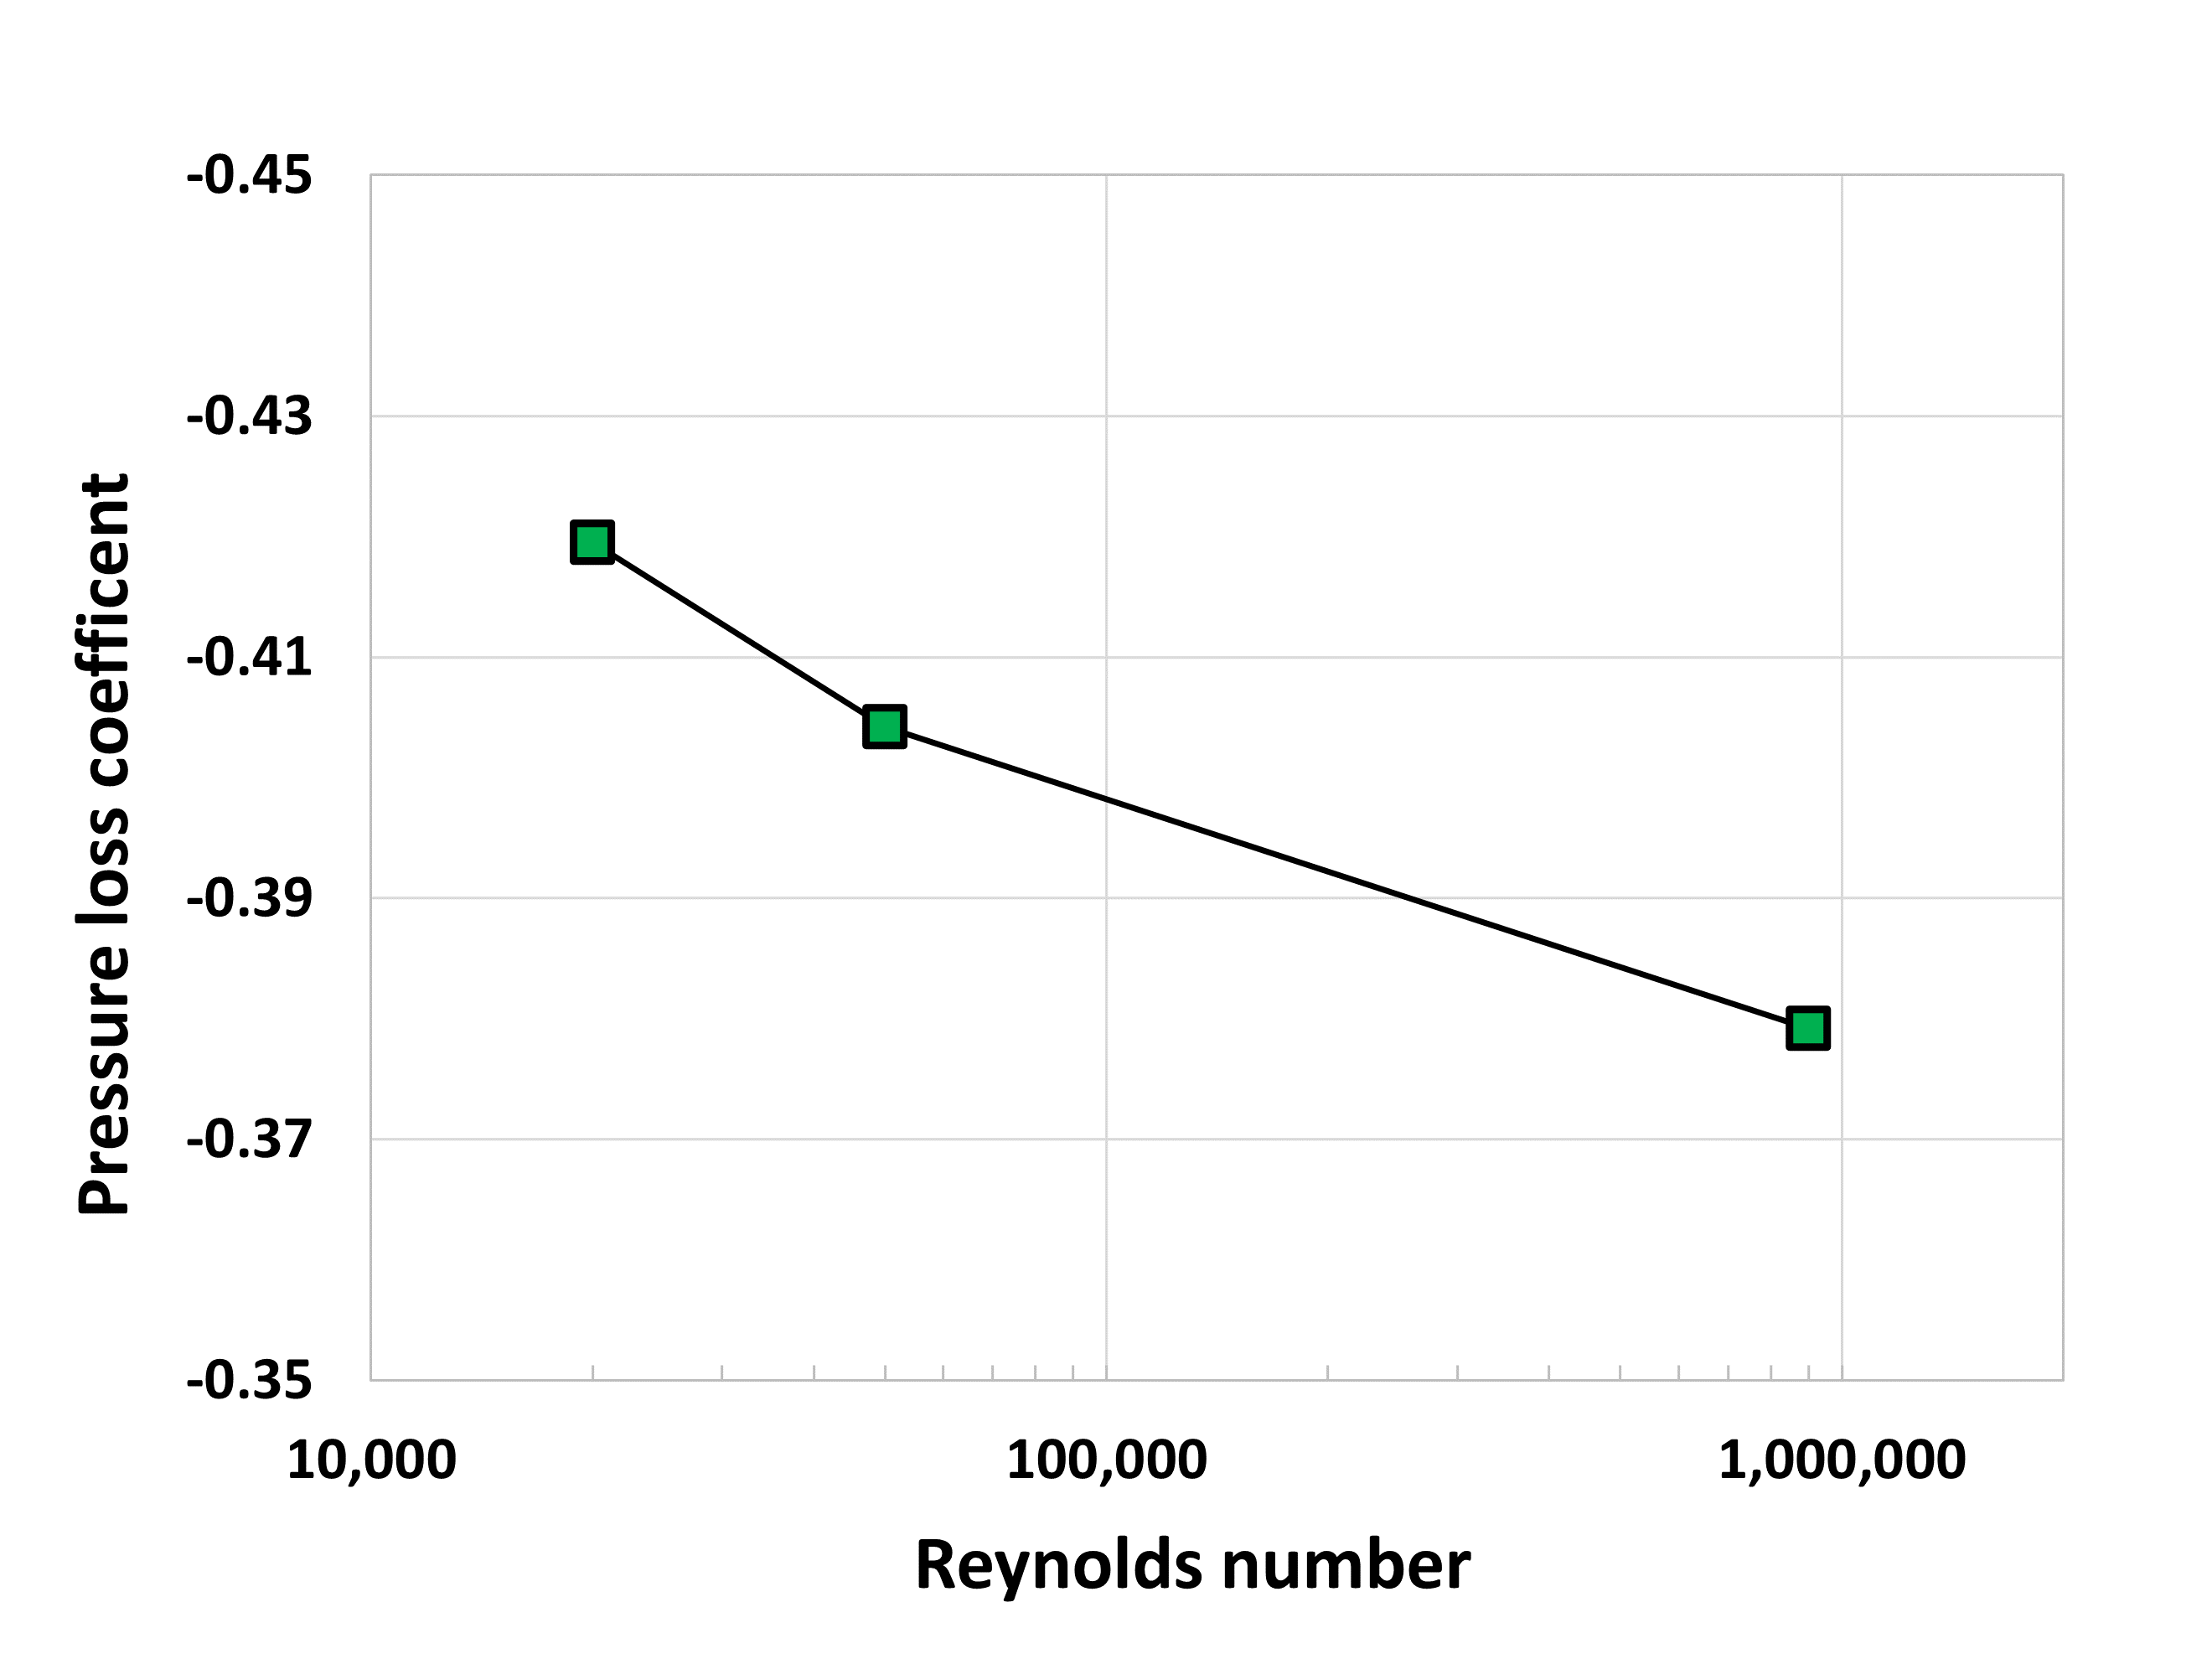
\includegraphics[width=0.6\textwidth]{./figures/pressure_loss.png}
\caption{The pressure loss coefficient due to the wall friction at different Reynolds numbers. }
\label{fig:pressure_loss}
\end{figure}

\begin{table} \centering \small
% \resizebox{0.48\textwidth}{!}{
 \begin{tabular}{ccccc} \hline \hline
   Re        & $\Delta P_t$   & $\Delta P_B$  & $\Delta P_F$  \\ \hline
   20,000    & 4.10E-02       & 2.81E-01      & -4.19E-01  \\
   50,000    & 5.62E-02       & 2.81E-01      & -4.04E-01  \\
   900,000   & 8.13E-02       & 2.81E-01      & -3.79E-01  \\
   \hline \hline
\end{tabular}
 \caption{The summary of pressure changes.}
 \label{tab:full core}
\end{table}



\subsection{Case study II: flow entering the pin bundle}
\label{sec:results2}

The second case study aims to test a novel simulation framework, NekNek, and demonstrate its usefulness in complex engineering geometries. A two-step approach is employed here: (i) a 2D backward facing step (BFS) case is first simulated to verify the NekNek performance; and (ii) the application of NekNek in simulating the flow entering a 7-pin fuel pin bundle geometry. The BFS case is selected because of the complex flow physics expected, such as the separation and shear flow. The BFS domain used in NekNek testing consists of two subchannels: an inlet with a length of 5.5 (0 to 5.5) and an outlet with a length of 20.0 (4.5 to 24.5) as shown in Figure~\ref{fig:bfs_domain}; two subdomains have an overlapped region from 4.5 to 5.5. The step height is 1.0 and a constant inflow velocity condition is given at the inlet face. The corresponding Reynolds number is 5,000. In addition to the NekNek test, a reference case is computed with the regular Nek5000 approach in an integral BFS domain. 


\begin{figure}[!ht]
\centering
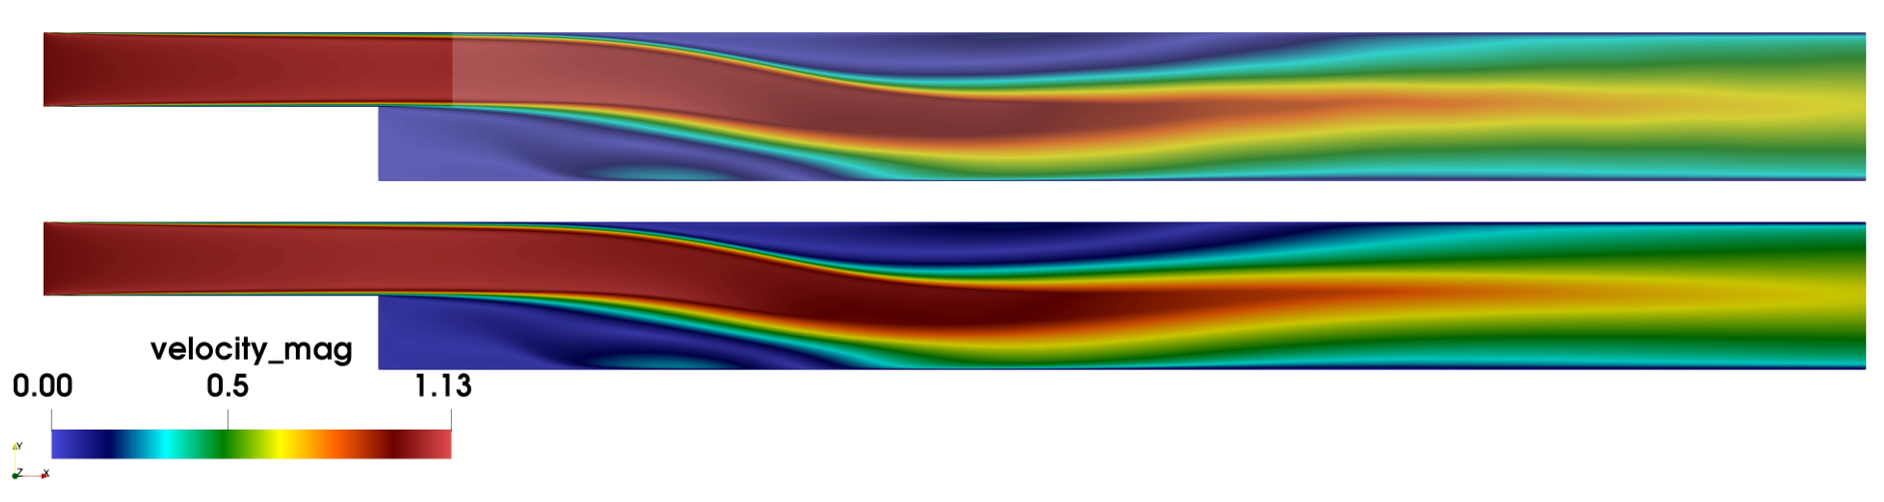
\includegraphics[width=0.9\textwidth]{./figures/bfs_vel.png}
\caption{The steady-state velocity field in decomposed NekNek subdomains (top) and the integral reference domain (bottom). }
\label{fig:bfs_domain}
\end{figure}

It is already qualitatively confirmed in Figure~\ref{fig:bfs_domain} that the NekNek approach can reproduce the overall flow behaviors as compared to those from the integral domain with regular Nek5000 approach. The boundary layer detachment is observed at the step edge. 
A re-circulation zone is created after the step and the flow eventually reattaches at roughly the same downstream location. A further scrutiny is carried out to compare the local data extracted. Figure~\ref{fig:bfs_results} compares the streamwise velocity and the turbulent kinetic energy along the line, $y=1.5$, throughout the BFS. 
Nearly identical results are produced from the NekNek approach and regular Nek5000 approach, which is a strong indicator of NekNek consistency. Smooth transition is observed for the quantities of interest over the overlapped region. 
It is worthwhile to point out that the continuity of pressure is not kept over subdomains as illustrated in Figure~\ref{fig:bfs_pressure}. Instead, the pressure gradient is strictly preserved, which is of paramount importance in incompressible flow solver. If one shifts the original pressure profile in the inlet region (i.e. the blue curve) down, it can perfectly match the pressure transition at the corresponding location in the integral domain (represented by the green curve). 

\begin{figure}[!ht]
\centering
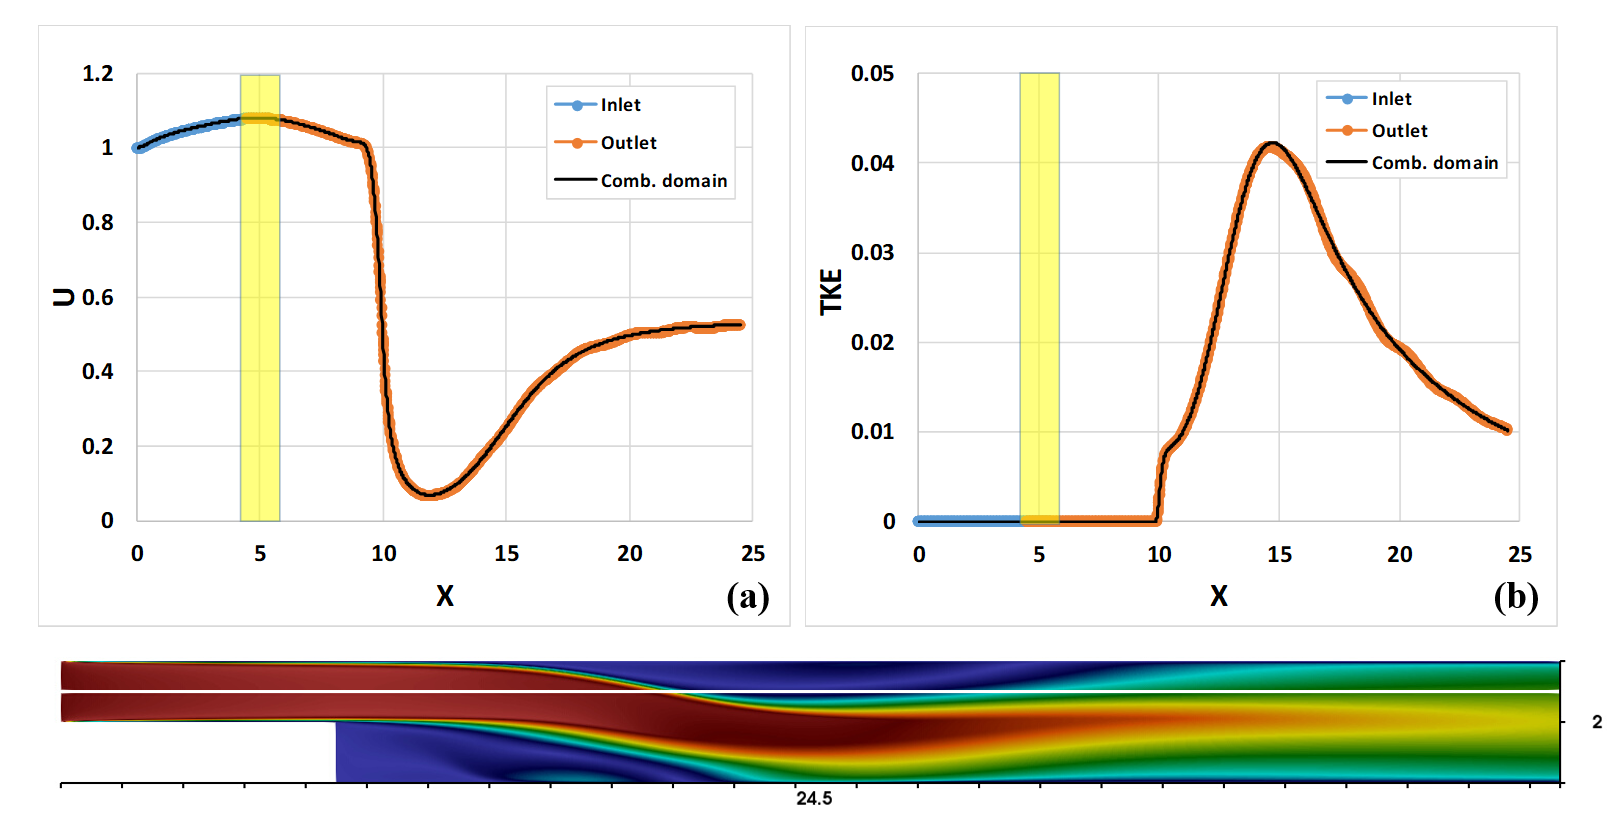
\includegraphics[width=0.8\textwidth]{./figures/bfs_neknek_results.png}
\caption{The steady-state profiles of streamwise velocity (U) and the turbulent kinetic energy (TKE) along the line ($y=1.5$). The yellow band indicates the bounds of overlapped region between subdomains. }
\label{fig:bfs_results}
\end{figure}

\begin{figure}[!ht]
\centering
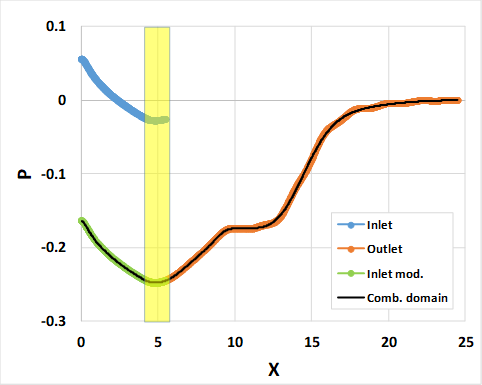
\includegraphics[width=0.6\textwidth]{./figures/bfs_neknek_pressure.png}
\caption{The steady-state pressure distribution along the line ($y=1.5$). }
\label{fig:bfs_pressure}
\end{figure}

As the next step, the NekNek is applied to simulate the flow entering the fuel pin bundle. A prototypical fuel bundle proposed for the SFR consists of 217 pins, and a simplified 7-pin bundle is considered here. The 7-pin bundle is adequate for the testing purpose and offers a much shorter turnaround time. 
As shown in Figure~\ref{fig:bundle_domain}, the geometry can be divided into two partitions: an upper subdomain contains the pin bundle and supporting structures, and a lower subdomain which is a vertical channel. 
The two subdomains overlap at the shared boundary illustrated in Figure~\ref{fig:bundle_domain} by the line between the upper subdomain (in red) and the lower subdomain (in blue). Two simultaneous simulation sessions are carried out in NekNek coupling for the flow in upper and lower subdomains, and the flow information is exchanged at the overlapping interface. Meanwhile, the integral domain is also simulated here with the regular Nek5000 approach to serve as the reference. The primary quantity of interest in this study is the pressure change when flow enters the fuel pin bundle. 

\begin{figure}[!ht]
\centering
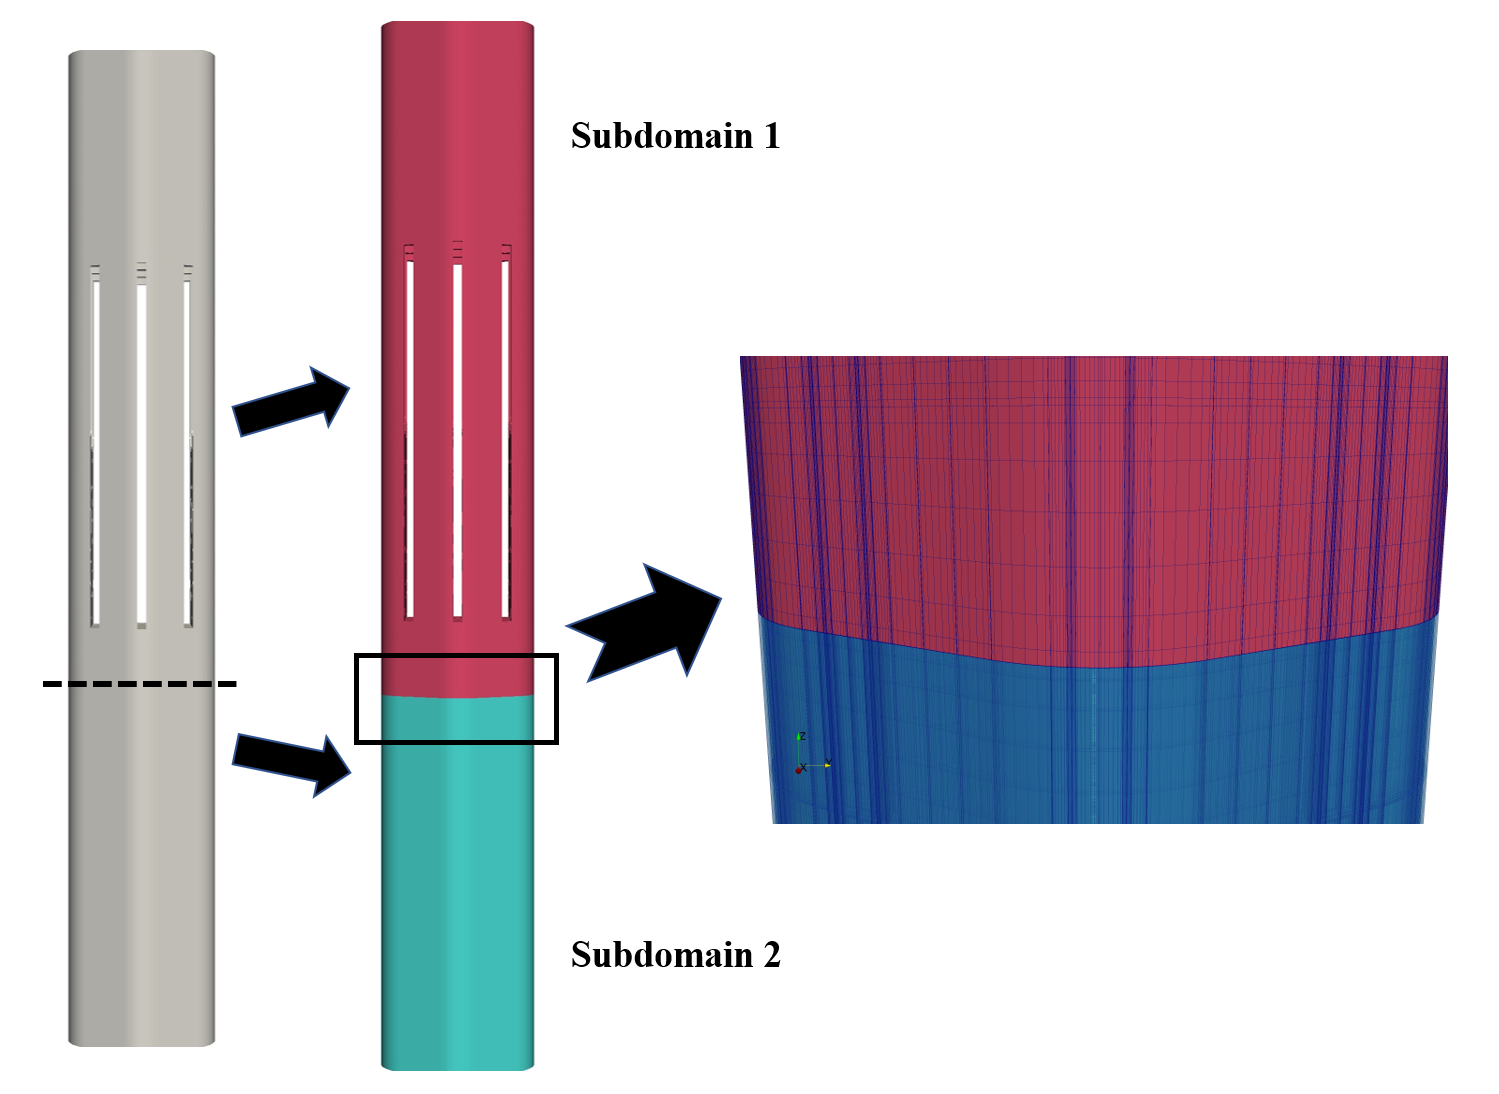
\includegraphics[width=0.8\textwidth]{./figures/bundle_neknek_domain.png}
\caption{The integral domain for the 7-pin demonstration case and the corresponding subdomains utilized in NekNek coupling. }
\label{fig:bundle_domain}
\end{figure}

The quasi-steady-state streamwise velocity distribution is showed in Figure~\ref{fig:bundle_vel}. 
The velocity profiles are almost identical except for the slight difference of unsteady wakes induced by supporting structures in the upper domain. A significant acceleration is observed due to the flow passage narrowing as the flow enters the fuel pin bundle. Following the same analysis strategy in the case study I, the total pressure change/loss is -9.832 in the integral domain while the pressure changes from two subdomains are -9.734 and -0.117 respectively. 
An excellent agreement is obtained again for the pressure data with only a 0.2\% deviation. Although extended verification efforts may still be needed, the consistency observed here is promising and the related efforts serve as an important stepping stone towards the NekNek application in more realistic/challenging engineering problems. 

\begin{figure}[!ht]
\centering
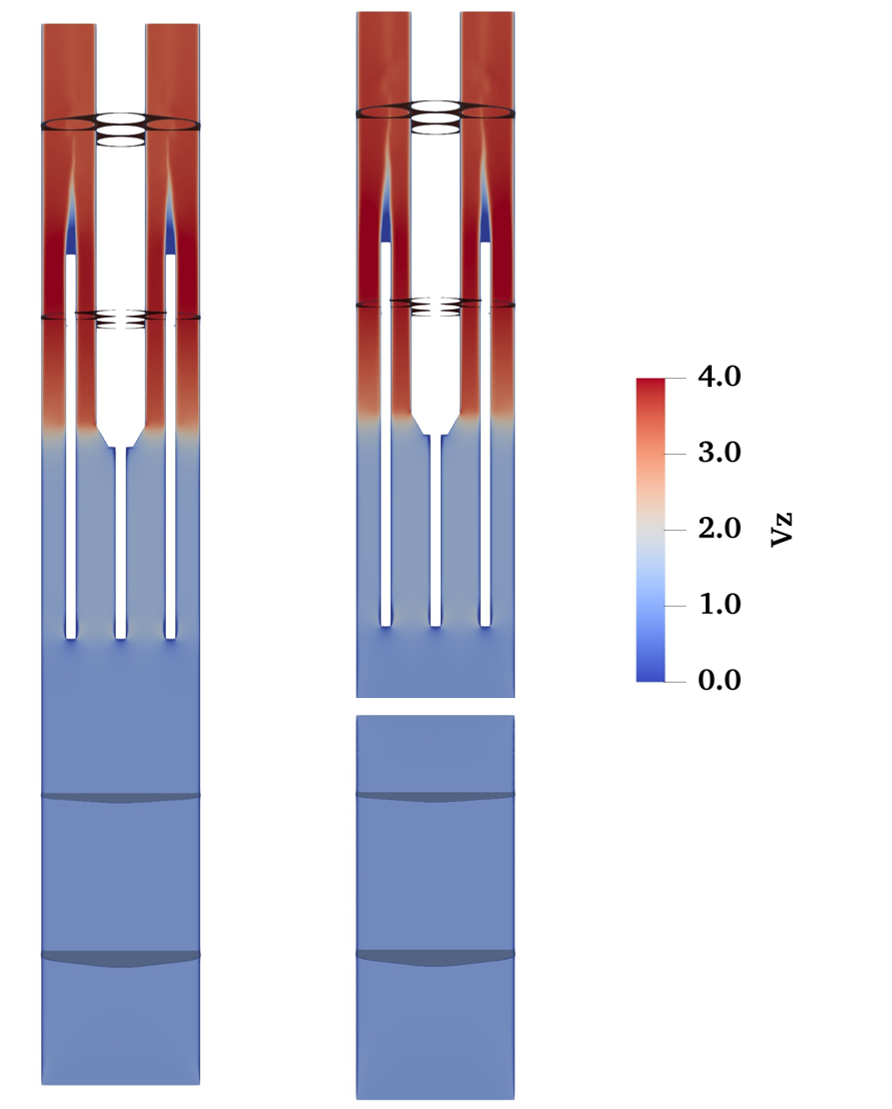
\includegraphics[width=0.5\textwidth]{./figures/bundle_neknek_results.png}
\caption{The quasi-steady-state streamwise velocity from the integral domain (left) and NekNek subdomains (right). }
\label{fig:bundle_vel}
\end{figure}
